% ------------------------------------------------------------------------------
% TYPO3 Version 10.1 - What's New (English Version)
%
% @author	Michael Schams <schams.net>
% @license	Creative Commons BY-NC-SA 3.0
% @link		http://typo3.org/download/release-notes/whats-new/
% @language	English
% ------------------------------------------------------------------------------

\section{Changes for Integrators}
\begin{frame}[fragile]
	\frametitle{Changes for Integrators}

	\begin{center}\huge{Chapter 2:}\end{center}
	\begin{center}\huge{\color{typo3darkgrey}\textbf{Changes for Integrators}}\end{center}

\end{frame}

% ------------------------------------------------------------------------------
% Feature | 89102 | Read settings for sites from <config>/sites/<siteIdentifier>/settings.yaml
%
%\begin{frame}[fragile]
%	\frametitle{Changes for Integrators}
%	\framesubtitle{Site-specific Settings (1)}
%
%	% decrease font size for code listing
%	\lstset{basicstyle=\smaller\ttfamily}
%
%	\begin{itemize}
%		\item A YAML file can provide site specific variables independent of the current context.
%
%		\item Place the file in the site configuration folder:\newline
%			\texttt{<config>/sites/<siteIdentifier>/settings.yaml}
%
%		\item For example:
%
%\begin{lstlisting}
%Vendor:
%   MyExtension:
%      storagePid: 1
%      limit: 15
%\end{lstlisting}
%
%	\end{itemize}
%
%\end{frame}
%
% ------------------------------------------------------------------------------
% Feature | 89102 | Read settings for sites from <config>/sites/<siteIdentifier>/settings.yaml
%
%\begin{frame}[fragile]
%	\frametitle{Changes for Integrators}
%	\framesubtitle{Site-specific Settings (2)}
%
%	% decrease font size for code listing
%	\lstset{basicstyle=\smaller\ttfamily}
%
%	\begin{itemize}
%		\item Settings can be accessed in TypoScript:
%
%\begin{lstlisting}
%plugin.tx_example.storagePid = {$Vendor.MyExtension.storagePid}
%\end{lstlisting}
%
%		\item Settings can also be accessed in PHP using the \texttt{Site} object:
%
%\begin{lstlisting}
%$settings = $site->getSettings();
%$storagePid = $settings['MyVendor']['MyExtension']['storagePid'];
%\end{lstlisting}
%
%	\end{itemize}
%
%\end{frame}

% ------------------------------------------------------------------------------
% Feature | 89227 | Ask for email address while installing TYPO3

\begin{frame}[fragile]
	\frametitle{Changes for Integrators}
	\framesubtitle{Administrator Email Address}

	\begin{columns}[T]
		\begin{column}{.04\textwidth}
		\end{column}
		\begin{column}{.38\textwidth}

			An email address can now be entered as part of the installation process.
			This address is used for the initial administrator backend user.

			\vspace{0.2cm}

			The same option exists in the Install Tool's Maintenance module
			\textbf{Create Administrative User}.

		\end{column}
		\begin{column}{.58\textwidth}
			\vspace{-0.3cm}
			\begin{figure}
				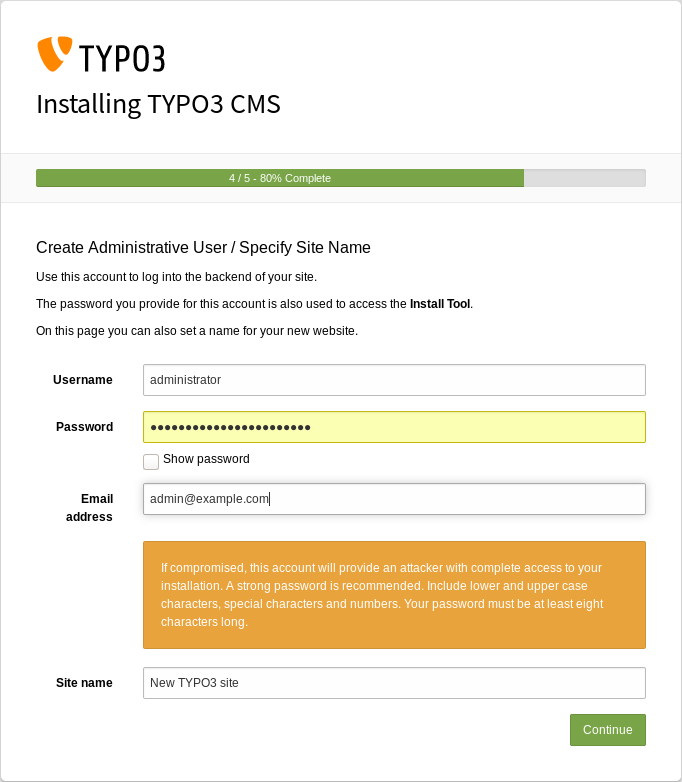
\includegraphics[width=0.70\linewidth]{ChangesForIntegrators/89227-EmailAddressDuringInstallation.png}
			\end{figure}
		\end{column}
	\end{columns}

\end{frame}

% ------------------------------------------------------------------------------
% Feature | 89229 | Cache Preset for Settings in Maintenance Area

% TRANSLATORS, PLEASE BE AWARE:
% We already included this slide in the 10.0 What's New Slides! However, the
% feature #89229 was removed from the TYPO3 core shortly before version 10.0 was
% published. Therefore, you possibly don't need to translate this slide again
% (just copy the text from the previous What's New Slides (search for the term
% "Cache Storage Type" in file ChangesForIntegrators.tex).

\begin{frame}[fragile]
	\frametitle{Changes for Integrators}
	\framesubtitle{Cache Storage Type (1)}

	\begin{itemize}

		\item TYPO3 features a flexible caching system with a default configuration
			that is ideal for most use cases.
		\item The storage type can now be configured to fine-tune the caches and
			increase performance depending on the individual environment.

			\begin{itemize}
				\item Choose the \textbf{database} storage for a standard environment
					or if a network file system (NFS) is used for example.
				\item Choose the \textbf{file system} if a distributed database setup
					is used for example.
				\item Choose \textbf{custom cache settings} to configure the storage
					type for each cache independently.
			\end{itemize}

		\item For more complex installations, memory-based caches such as
			\href{https://redis.io/}{Redis}
			or
			\href{https://memcached.org/}{Memcached}
			should be considered.

	\end{itemize}

\end{frame}

% ------------------------------------------------------------------------------
% Feature | 89229 | Cache Preset for Settings in Maintenance Area

% TRANSLATORS, PLEASE BE AWARE:
% We already included this slide in the 10.0 What's New Slides! However, the
% feature #89229 was removed from the TYPO3 core shortly before version 10.0 was
% published.
%
% On this slide, the path to the function in the backend needs to be adjusted:
% ADMIN TOOLS -> Settings -> Configuration Presets

\begin{frame}[fragile]
	\frametitle{Changes for Integrators}
	\framesubtitle{Cache Storage Type (2)}

	\begin{itemize}

		\item Backend: \textbf{ADMIN TOOLS} \ding{223}\hspace{0.1cm}\textbf{Settings} \ding{223}\hspace{0.1cm}\textbf{Configuration Presets}:
		\end{itemize}

	\begin{figure}
		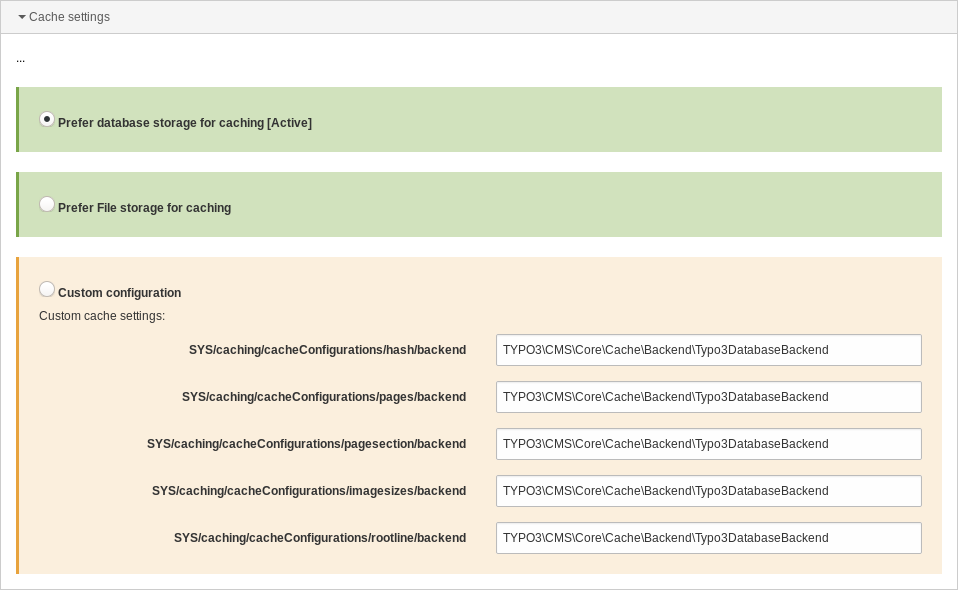
\includegraphics[width=0.60\linewidth]{ChangesForIntegrators/89229-CachePresetForSettingsInMaintenanceArea.png}
	\end{figure}

\end{frame}

% ------------------------------------------------------------------------------
% Feature | 89142 | Create site configuration if page is created on root level

\begin{frame}[fragile]
	\frametitle{Changes for Integrators}
	\framesubtitle{Site Configuration}

	\begin{itemize}
		\item When a new page is created on the root level, a standard site
			configuration is automatically generated with it.
		\item As a result, a basic TYPO3 site can be set up quickly.
		\item The site configuration features:

			\begin{itemize}
				\item a pre-defined identifier (e.g. \texttt{site-42-a1d0c6e83f})
				\item an entry point (e.g. \texttt{https://example.com/site-42})
				\item a default language (e.g. \texttt{English})
			\end{itemize}

	\end{itemize}

\end{frame}

% ------------------------------------------------------------------------------
% Feature | 89090 | Reports for conflicting redirects

\begin{frame}[fragile]
	\frametitle{Changes for Integrators}
	\framesubtitle{Conflicting Redirects (1)}

	\begin{itemize}
		\item A new Symfony command has been introduced to detect redirects
			that conflict with page URLs.
		\item Execute the command in the CLI:\newline
			\smaller
				(optional parameter \texttt{-}\texttt{-site} limits the check to a specific site)
			\normalsize
	\end{itemize}

	\begin{figure}
		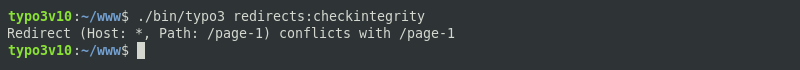
\includegraphics[width=0.90\linewidth]{ChangesForIntegrators/89090a-ReportsForConflictingRedirects.png}
	\end{figure}

	\begin{itemize}
		\item The command is also available as a scheduler task:
	\end{itemize}

	\begin{figure}
		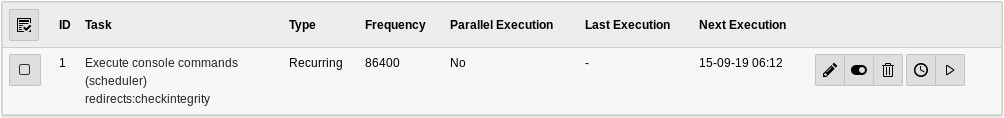
\includegraphics[width=0.90\linewidth]{ChangesForIntegrators/89090b-ReportsForConflictingRedirects.png}
	\end{figure}

\end{frame}

% ------------------------------------------------------------------------------
% Feature | 89090 | Reports for conflicting redirects

\begin{frame}[fragile]
	\frametitle{Changes for Integrators}
	\framesubtitle{Conflicting Redirects (2)}

	\begin{itemize}
		\item A list of detected conflicting redirects can also be accessed in the Reports module:
	\end{itemize}

	\begin{figure}
		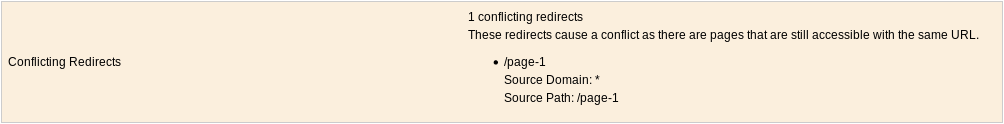
\includegraphics[width=0.90\linewidth]{ChangesForIntegrators/89090c-ReportsForConflictingRedirects.png}
	\end{figure}

	\begin{itemize}
		\item
			\small\textbf{Note:}
				The command needs to be executed again to "reset" the list.
				Solving the issue (e.g. by removing the redirect) does not clear the list.
			\normalsize
	\end{itemize}

\end{frame}

% ------------------------------------------------------------------------------
% Feature | 89010 | Introduce Site Configuration for Distribution Packages

\begin{frame}[fragile]
	\frametitle{Changes for Integrators}
	\framesubtitle{Distribution Packages}

	% decrease font size for code listing
	\lstset{basicstyle=\tiny\ttfamily}

	\begin{itemize}
		\item Distributions can now provide site configuration file(s).

		\item Create a directory/file in the distribution package as follows:\newline
			\texttt{Initialisation/Site/<siteIdentifier>/config.yaml}

		\item Similar to assets, which are moved to \texttt{fileadmin/},\newline
			site configurations are moved to the \texttt{config/} folder.

		\item If the target directory already exists, no change is made to the existing configuration.
	\end{itemize}

\end{frame}

% ------------------------------------------------------------------------------
% Feature | 88318 | Display Application Context in CLI

\begin{frame}[fragile]
	\frametitle{Changes for Integrators}
	\framesubtitle{Application Context in CLI}

	\begin{itemize}
		\item The current Application Context is now shown next to the
			TYPO3 version number in CLI requests:
	\end{itemize}

	\begin{figure}
		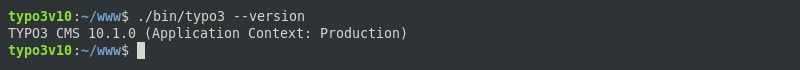
\includegraphics[width=0.90\linewidth]{ChangesForIntegrators/88318-DisplayApplicationContextInCli.png}
	\end{figure}

\end{frame}

% ------------------------------------------------------------------------------
% Feature | 87525 | Add api=1 option in VimeoRenderer

\begin{frame}[fragile]
	\frametitle{Changes for Integrators}
	\framesubtitle{Vimeo Video Rendering}

	% decrease font size for code listing
	\lstset{basicstyle=\smaller\ttfamily}

	\begin{itemize}
		\item The parameter \texttt{api=1} in Vimeo video URLs allows API interactions with the video player (e.g. adding buttons to control the video).
		\item Integrators can now set this parameter in two different ways.

		\begin{itemize}
			\item Using TypoScript:

\begin{lstlisting}
lib.contentElement.settings.media.additionalConfig.api = 1
\end{lstlisting}

			\item In Fluid using the Media-ViewHelper:

\begin{lstlisting}
<f:media
  file="{file}"
  alt="{file.properties.alternative}"
  title="{file.properties.title}"
  additionalConfig="{api: 1}"
/>
\end{lstlisting}

		\end{itemize}
	\end{itemize}

\end{frame}

% ------------------------------------------------------------------------------
% Feature | 86670 | Make default action in DragUploader adjustable

\begin{frame}[fragile]
	\frametitle{Changes for Integrators}
	\framesubtitle{File Uploads}

	% decrease font size for code listing
	\lstset{basicstyle=\smaller\ttfamily}

	\begin{itemize}
		\item It is now possible to configure the default action when uploading files in the file list module using drag'n drop.
		\item User TSConfig:

\begin{lstlisting}
# Set default to replace:
options.file_list.uploader.defaultAction = replace

# Set default to rename:
options.file_list.uploader.defaultAction = rename

# Set default to cancel:
options.file_list.uploader.defaultAction = cancel
\end{lstlisting}

	\end{itemize}

\end{frame}

% ------------------------------------------------------------------------------
% Feature | 84250 | Separately enable / disable "Add media by URL" and "Select & upload files"

\begin{frame}[fragile]
	\frametitle{Changes for Integrators}
	\framesubtitle{Media Element Buttons}

	% decrease font size for code listing
	\lstset{basicstyle=\tiny\ttfamily}

	\begin{itemize}
		\item Buttons \textbf{"Add media by URL"} and \textbf{"Select \& upload files"}
			can now be enabled/disabled independently from each other.
	\end{itemize}

	\begin{figure}
		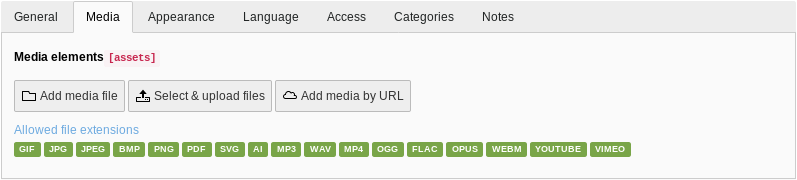
\includegraphics[width=0.75\linewidth]{ChangesForIntegrators/84250-EnableDisableMediaButtons.png}
	\end{figure}

	\begin{itemize}
		\item The example below hides both buttons:

\begin{lstlisting}
$GLOBALS['TCA']['pages']['columns']['media']['config']['appearance'] = [
  'fileUploadAllowed' => false,
  'fileByUrlAllowed' => false,
];
\end{lstlisting}

	\end{itemize}

\end{frame}

% ------------------------------------------------------------------------------
% Feature | 88441 | Show configuration of USER_INT objects in adminpanel

\begin{frame}[fragile]
	\frametitle{Changes for Integrators}
	\framesubtitle{Admin Panel}

	\begin{itemize}
		\item The Admin Panel features a new panel \textbf{USER\_INT} under the "Info" module.
	\end{itemize}

	\begin{figure}
		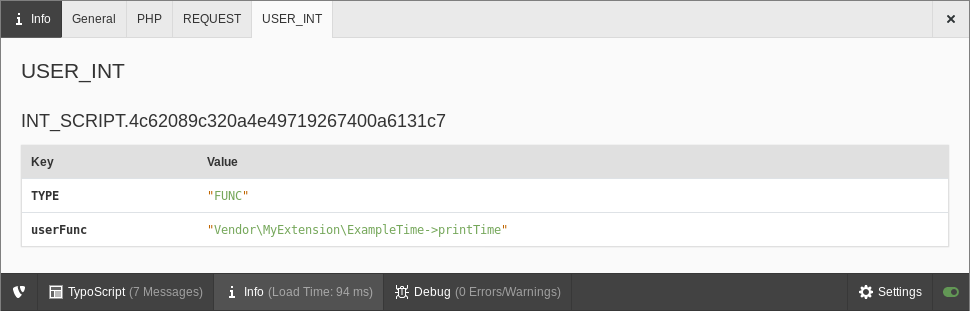
\includegraphics[width=0.90\linewidth]{ChangesForIntegrators/88441-ShowUserIntObjectsInAdminPanel.png}
	\end{figure}

\end{frame}

% ------------------------------------------------------------------------------
